\documentclass[../analysisII_notes.tex]{subfiles}
\begin{document}
\section{Aula 03 - 10 de Março, 2025}
\subsection{Motivações}
\begin{itemize}
	\item Introdução à construção de integral de Darboux;
	\item Somas superiores e inferiores;
	\item Integrais de Riemann.
\end{itemize}
\subsection{Integrais Superiores e Inferiores - Parte 1}
Nesta aula, entraremos de vez na ementa do curso, começando pela estruturação de Darboux das integrais pelas somas inferior e superior.

A fim de concluir este objetivo, lembremos um conceito necessário para estudar as integrais próprias:
\begin{tcolorbox}[
		skin=enhanced,
		title=Lembrete!,
		after title={\hfill Imagem de Função},
		fonttitle=\bfseries,
		sharp corners=downhill,
		colframe=black,
		colbacktitle=yellow!75!white,
		colback=yellow!30,
		colbacklower=black,
		coltitle=black,
		%drop fuzzy shadow,
		drop large lifted shadow
	]
	Dado um subconjunto X da reta real e \(f:X\rightarrow \mathbb{R}\), ela é dita limitada se seu conjunto imagem é limitado, ou seja,
	\[
		\mathrm{Im}(f) \equiv f(X) \coloneqq \{f(x):x \in X\}
	\]
	é limitado. Graficamente, isto normalmente significa que toda a sua imagem está contida dentro de um certo intervalo de tamanho fixo no eixo y.
\end{tcolorbox}

Convencionamos, para uma função \(f:[a, b]\rightarrow \mathbb{R}\) limitada, a notação:
\[
	m\coloneqq \inf_{}(f) = \inf_{a\leq x\leq b}\{f(x)\}
\]
e
\[
	M\coloneqq \sup_{}(f) = \sup_{a\leq x\leq b}\{f(x)\}
\]

\begin{figure}[H]
	\begin{center}
		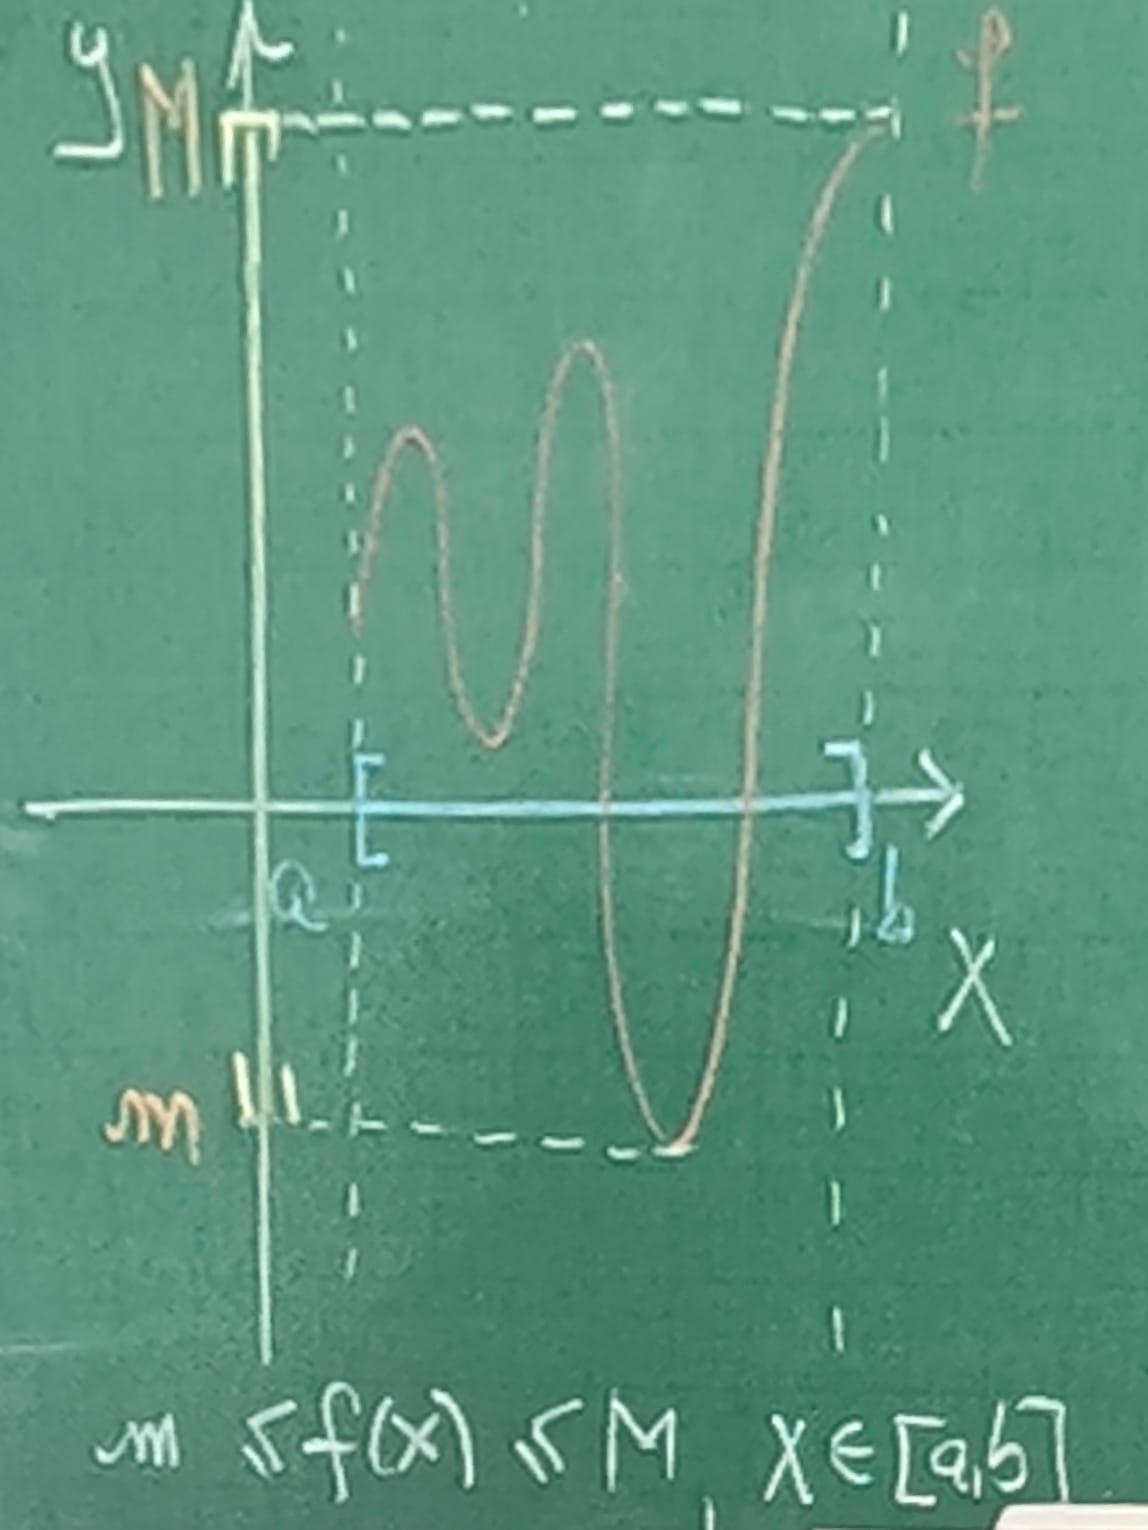
\includegraphics[height=0.3\textheight, width=0.3\textwidth, keepaspectratio]{./Images/bounded_03.png}
	\end{center}
	\caption{função limitada entre m e M, em que m e M são duas constantes reais.}
	\label{bdd03}
\end{figure}

\begin{figure}[H]
	\begin{center}
		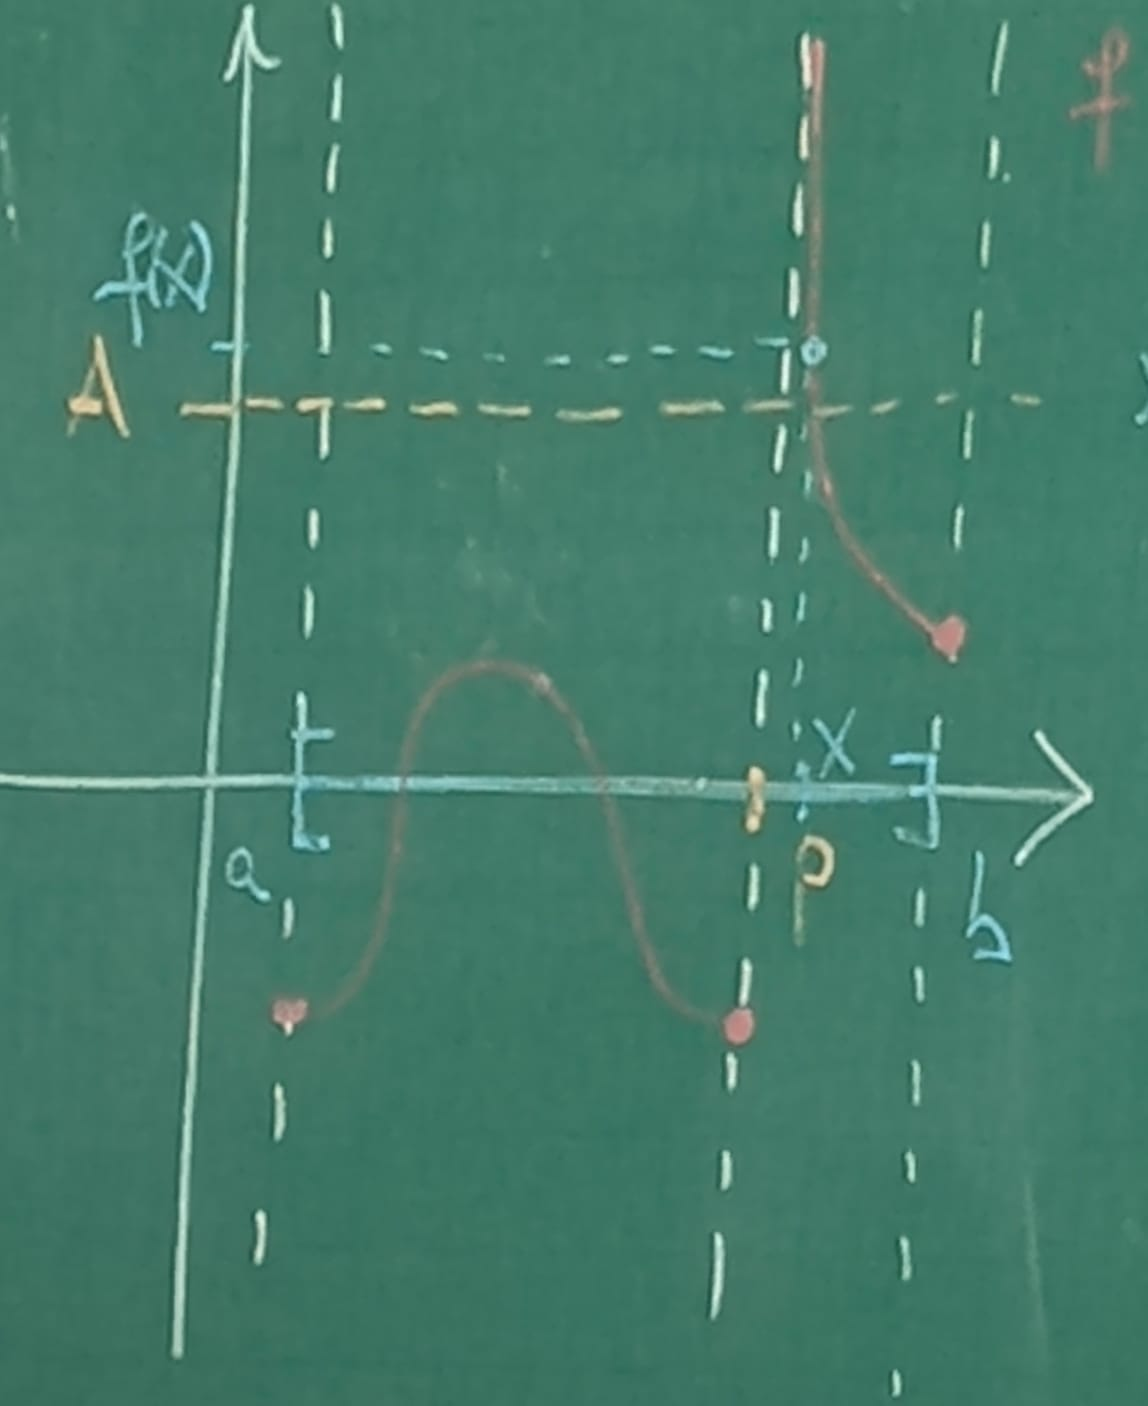
\includegraphics[height=0.3\textheight, width=0.3\textwidth, keepaspectratio]{./Images/unbounded_03.png}
	\end{center}
	\caption{função ilimitada: conforme x se aproxima de p pela direita, a função tende ao infinito; em termos matemáticos, \(\lim_{x\to p^{+}}f(x)=\infty\)}
	\label{ubdd03}
\end{figure}

Vejamos alguns componentes do vocabulário utilizado na abordagem de Darboux, fixando um intervalo \([a, b]\) e uma função \(f:[a, b]\rightarrow \mathbb{R}\) limitada:
\begin{def*}
	Uma \textbf{partição de [a, b]} é um subconjunto finito \(\mathcal{P} = \{t_{0}, t_1, t_2, \dotsc , t_{n}\}\subseteq [a, b]\) que contenha os extremos a e b. Escrevemos:
	\[
		\mathcal{P}: a = t_{0}<t_1 <t_2 <\dotsc <t_{n}=b.\quad \square
	\]
\end{def*}
Dada uma família de índices finitos \(i = 1, 2, \dotsc , n\), escreveremos
\[
	I_{i}\coloneqq [t_{i-1}, t_{i}]
\]
para o i-ésimo subintervalo de \(\mathcal{P}\).

Observe que, se somarmos os comprimentos de todos os subintervalos, teremos uma série telescópica da forma
\[
	\sum\limits_{i=1}^{n}(t_{i}-t_{i-1}) = (t_1 - t_{0}) + (t_2 - t_1) + \dotsc + (t_{n-1} - t_{n-2}) + (t_{n} - t_{n-1}) = t_{n} - t_{0} = b - a,
\]
o que significa que, ao somar os tamanhos de todas os subintervalos de uma partição de [a, b], obtemos o tamanho do intervalo original.
Pode-se dizer, então, que particionar um intervalo ``preserva o tamanho dele''.

Denotamos o conjunto de todas as partições de [a, b] por \(\mathcal{P}([a, b])\). Com isso,
\begin{def*}
	Dadas duas partições \(\mathcal{P}, \mathcal{Q}\in \mathcal{P}([a, b])\), dizemos que \(\mathcal{Q}\) \textbf{refina} \(\mathcal{P}\) quando \(\mathcal{P}\) é um subconjunto de \(\mathcal{Q}\). \(\square\)
\end{def*}
\begin{example}
	Dada uma partição da forma
	\[
		\mathcal{P}: a = t_{0} < t_{1} < \dotsc < t_{n} = b,
	\]
	então \(\mathcal{Q} = \mathcal{P}\cup \{t'\}\), em que \(t'\) pertence a [a, b], refina \(\mathcal{P}\), como na figura abaixo.
	\begin{figure}[H]
		\begin{center}
			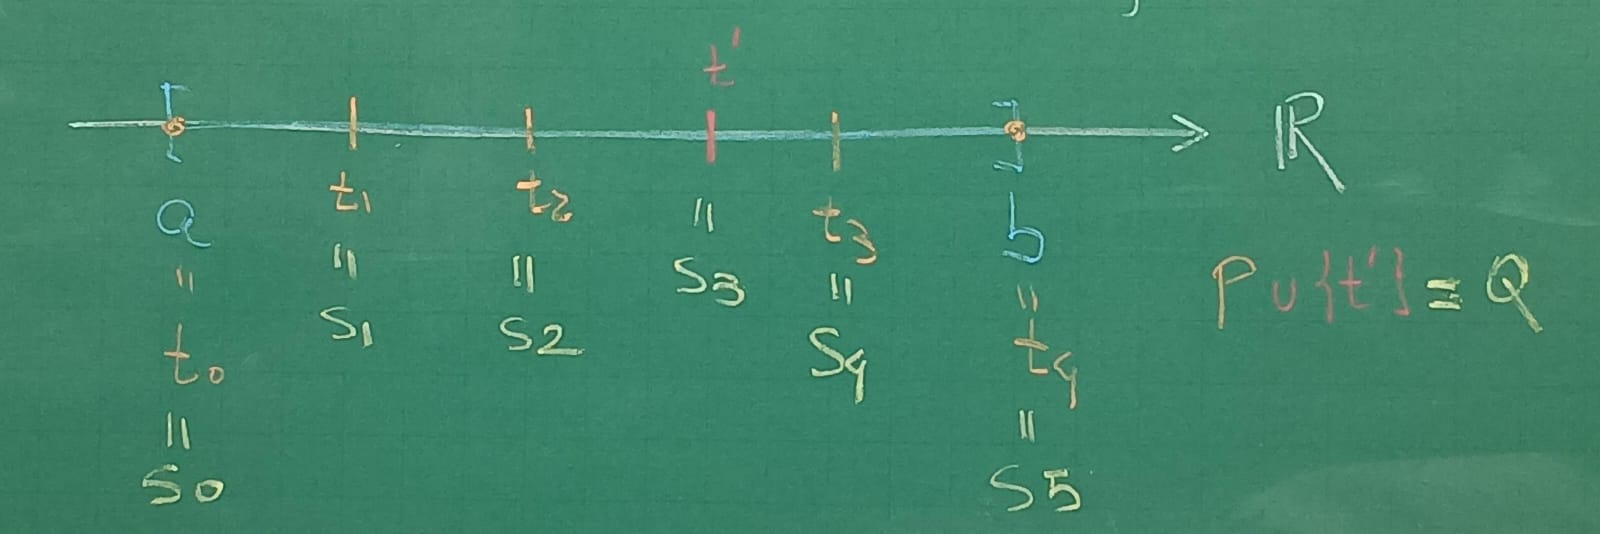
\includegraphics[height=\textheight, width=\textwidth, keepaspectratio]{./Images/partition_03.png}
		\end{center}
		\caption{ao refinar uma partição, adiciona-se um ponto a mais. Neste caso, a partição \(\mathcal{P}\), denotada pelos \(t_{i}\)'s, foi refinada ao acrescentar o ponto t', formando a nova partição \(\mathcal{Q}\).}
		\label{refine03}
	\end{figure}
\end{example}

Dada uma partição
\[
	\mathcal{P}: a = t_{0} < t_1 < t_2 <\dotsc <t_{n} = b,
\]
colocamos
\begin{align*}
	 & m_{i} = \inf_{}\{f(x):x\in I\}  \\
	 & M_{i} = \sup_{}\{f(x):x\in I\},
\end{align*}
em que \(i= 1, 2, \dotsc , n.\) Em outras palavras, estes símbolos denotam os menores e maiores valores para cada subintervalo da partição \(\mathcal{P}([a, b])\).
\begin{figure}[H]
	\begin{center}
		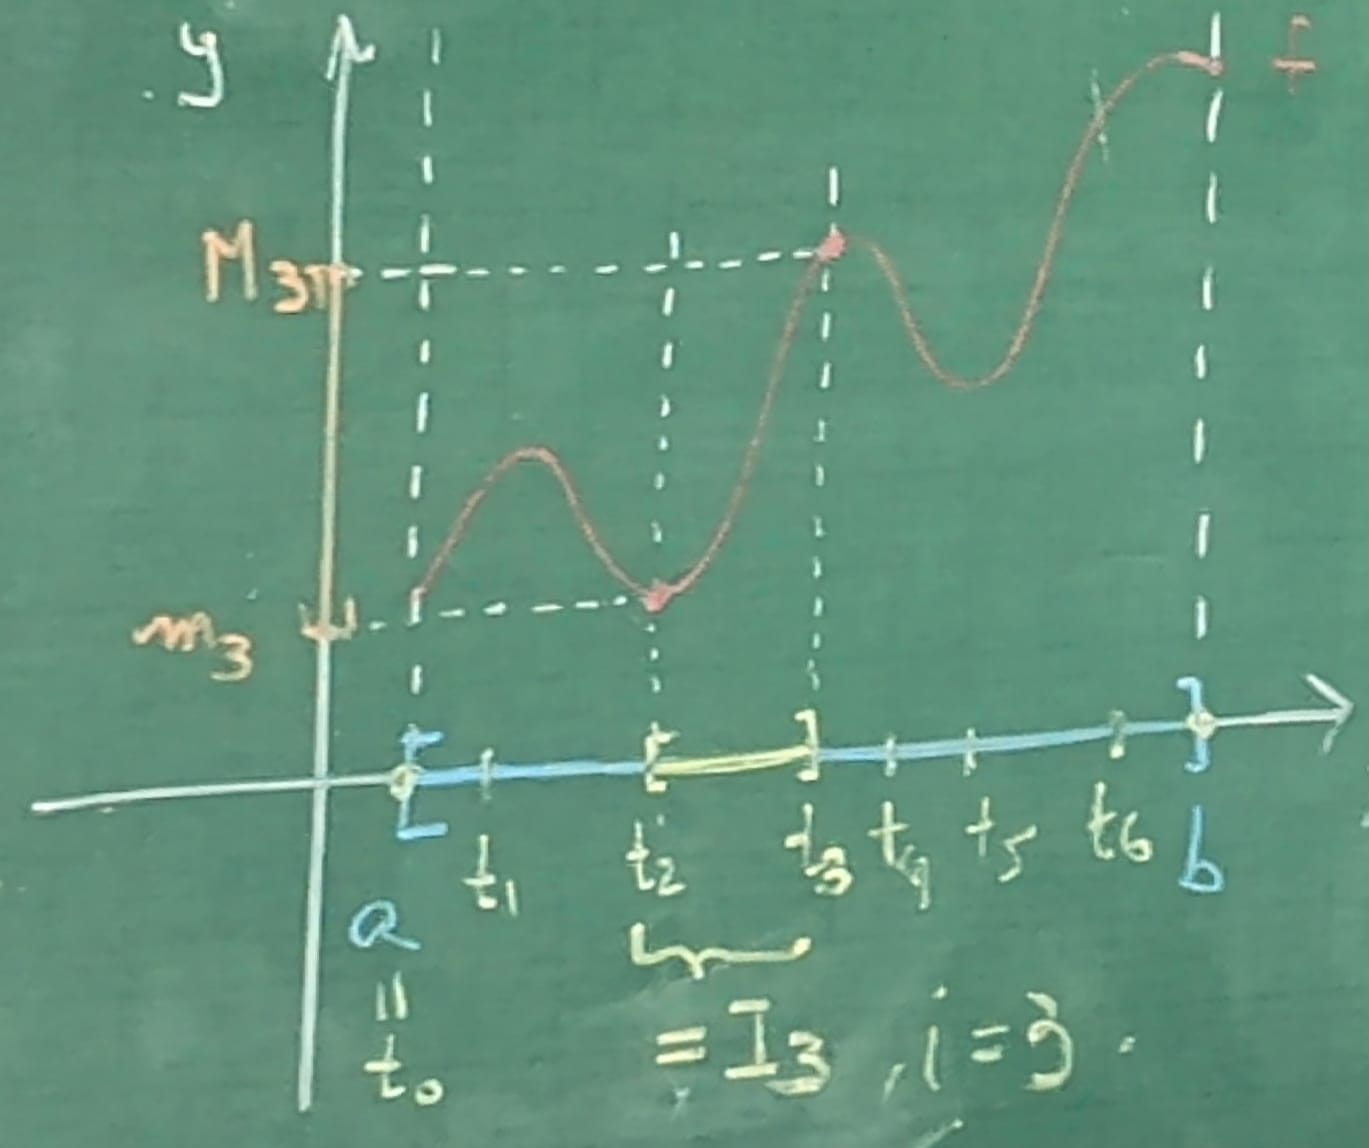
\includegraphics[height=0.5\textheight, width=0.5\textwidth, keepaspectratio]{./Images/supinf_partition_03.png}
	\end{center}
	\caption{ilustração de como cada subintervalo terá valores específicos de \(m_{i}\) e \(M_{i}\). Em particular, ele deixa bem claro como , para todo x nos subintervalos, \(m_{i}\leq f(x)\leq M_{i}\).}
	\label{supingf03}
\end{figure}

Agora sim, podemos finalmente definir a primeira parte da jornada até a integral de Riemann, as somas superior e inferior de uma função.
\begin{def*}
	Se \(f:[a, b]\rightarrow \mathbb{R}\) é limitada e
	\[
		\mathcal{P}: a = t_{1} < t_2 < \dotsc < t_{n} = b
	\]
	é um partição do intervalo \([a, b]\), definimos
	\begin{itemize}
		\item[I)] A \textbf{soma superior de f relativa a }\(\mathcal{P}\) por
		      \[
			      U(f; \mathcal{P}) = U(\mathcal{P}) = \sum\limits_{i=1}^{n}M_{i}(t_{i}-t_{i-1})
		      \]
		\item[II)] A \textbf{soma inferior de f relativa a }\(\mathcal{P}\) por
		      \[
			      L(f; \mathcal{P}) = \sum\limits_{i=1}^{n}m_{i}(t_{i}-t_{i-1}). \quad \square
		      \]
	\end{itemize}
\end{def*}
Ao olhar para esta definição em um bom desenho, nota-se que elas representam as áreas de retângulos!  No caso da soma superior, ele representa um retângulo que consome ``mais área'' do que a área embaixo da função. Em contrapartida, a soma inferior deixa cobre ``menos área'' do que a área abaixo de f.

\begin{figure}[H]
	\begin{center}
		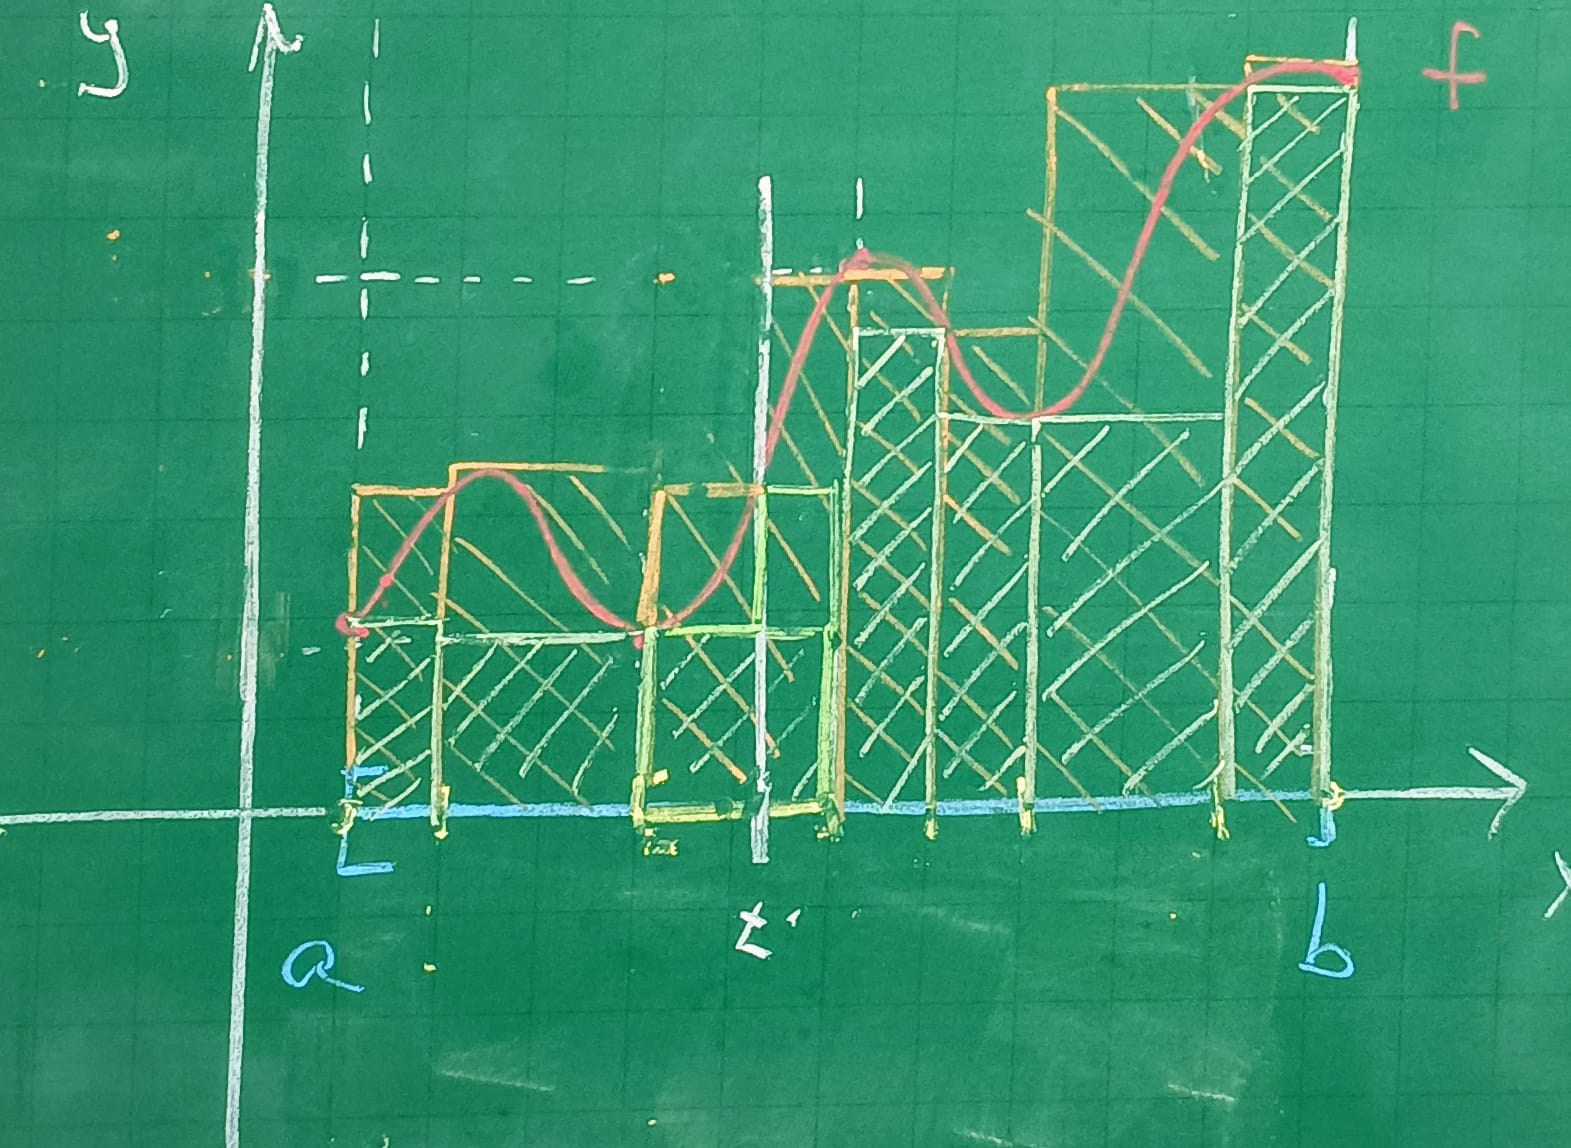
\includegraphics[height=0.6\textheight, width=0.6\textwidth, keepaspectratio]{./Images/sums_03.png}
	\end{center}
	\caption{em laranja, temos as somas superiores cobrindo mais área do que a da função em vermelho, e, em cinza, cobrindo menos. Conforme as partições são refinadas, as áreas passam a ficar mais similares à da função!}
	\label{uisums03}
\end{figure}

Observe que, fixada uma função \(f:[a, b]\rightarrow \mathbb{R}\) limitada, dada uma partição
\[
	\mathcal{P}:a = t_{0} < t_1 < \dotsc < t_{n} = b,
\]
temos:
\begin{itemize}
	\item[a)] Para qualquer \(i = 1, 2, \dotsc, n\), vale que \(m_{i}\) é maior que o m\footnote{Afinal, cada subintervalo é um subconjunto do intervalo maior, então podemos aplicar as propriedades do ínfimo de subconjuntos para obter essa desigualdade.}, Como consequência,
	      \[
		      m(t_{i}-t_{i-1}) \leq m_{i}(t-t_{i-1}),
	      \]
	      donde segue que
	      \[
		      m(b-a) = m \sum\limits_{i=1}^{n}(t_{i} - t_{i-1}) \leq \sum\limits_{i=1}^{n}m_{i}(t_{i}-t_{i-1}) = L(f; \mathcal{P}).
	      \]
	      Consequentemente, para qualquer partição \(\mathcal{P}\) do intervalo [a, b],
	      \[
		      m(b-a)\leq L(f; \mathcal{P}).
	      \]
	\item[b)] Por um processo análogo, vale que
	      \[
		      M_{i}\leq M \Rightarrow U(f; \mathcal{P}) \leq M(b-a).
	      \]
	\item[c)] Como o ínfimo do intervalo é menor que o supremo dele, o seguinte é verdade:
	      \[
		      m_{i}(t_{i}-t_{i-1}) \leq M_{i}(t_{i}-t_{i-1}) \Rightarrow L(f; \mathcal{P})\leq U(f; \mathcal{P})
	      \]
\end{itemize}

Juntando dos itens (a) ao (c), provamos a proposição que diz que
\begin{prop*}
	Se \(f:[a, b]\rightarrow \mathbb{R}\) for limitada e \(\mathcal{P}\) for uma partição do intervalo \([a, b]\), então
	\[
		m(b-a)\leq L(f; \mathcal{P}) \leq U(f; \mathcal{P}) \leq M(b-a).
	\]
\end{prop*}

Sob as hipóteses da proposição, os conjuntos das somas inferiores e das somas superiores são não-vazios e limitados, ou seja, pelo \hyperlink{lub_property}{\textit{axioma do supremo e ínfimo}}, eles têm supremo e ínfimo! Na forma de um corolário,
\begin{crl*}
	Definindo os seguintes conjuntos,
	\begin{align*}
		 & \sigma (f) = \{L(f; \mathcal{P}): \mathcal{P}\in \mathcal{P}([a, b])\}  \\
		 & \Sigma (f) = \{U(f; \mathcal{P}): \mathcal{P}\in \mathcal{P}([a, b])\},
	\end{align*}
	eles constituem conjuntos não-vazios e limitados.
\end{crl*}

Até o momento, fomos testando as coisas fixando uma certa partição; nessa linha, o próximo passo é variar as partições: ao invés de olhar apenas para \(\mathcal{P}\), passaremos a considerar as interações entre partições \(\mathcal{P}\) e \(\mathcal{Q}\) diferentes.

\begin{theorem*}
	Quando refinamos uma partição \(\mathcal{P}\) com uma outra \(\mathcal{Q}\):
	\begin{itemize}
		\item[1)] As somas superiores não aumentam (podem diminuir ou ficarem iguais):
		      \[
			      \mathcal{P}\subseteq \mathcal{Q}\Rightarrow U(f; \mathcal{Q})\leq U(f; \mathcal{P});
		      \]
		\item[2)] As somas inferiores não diminuem (podem aumentar ou ficarem iguais):
		      \[
			      \mathcal{P}\subseteq \mathcal{Q}\Rightarrow L(f; \mathcal{Q})\geq L(f; \mathcal{P}).
		      \]

	\end{itemize}
\end{theorem*}
\begin{proof*}
	A prova é dividida em duas etapas. Na primeira, olharemos para um refinamento bem simples da partição \(\mathcal{P}\), dado por
	\[
		\mathcal{Q} = \mathcal{P}\cup \{t'\}.
	\]
	Suponhamos, mais especificamente, que
	\[
		\mathcal{P}:a = t_{0} < t_{1} < t_2 < \dotsc < t_{n} = b
	\]
	e que \(t'\) está entre o k-ésimo ponto da partição e seu antecessor: \(t_{k-1}<t'<t_{k}\), para algum k entre 1 e n.

	Daí, vemos que
	\begin{align*}
		 & M' = \sup_{}\{f(x): t_{k-1}\leq x \leq t'\} \\
		 & M'' = \sup_{}\{f(x):t' \leq x \leq t_{k}\}
	\end{align*}
	separam o k-ésimo subintervalo em duas partes, o que leva-nos à conclusão de que tanto M' quanto M'' são menores ou iguais ao supremo do subintervalo, \(M_{k}\).

	\begin{figure}[H]
		\begin{center}
			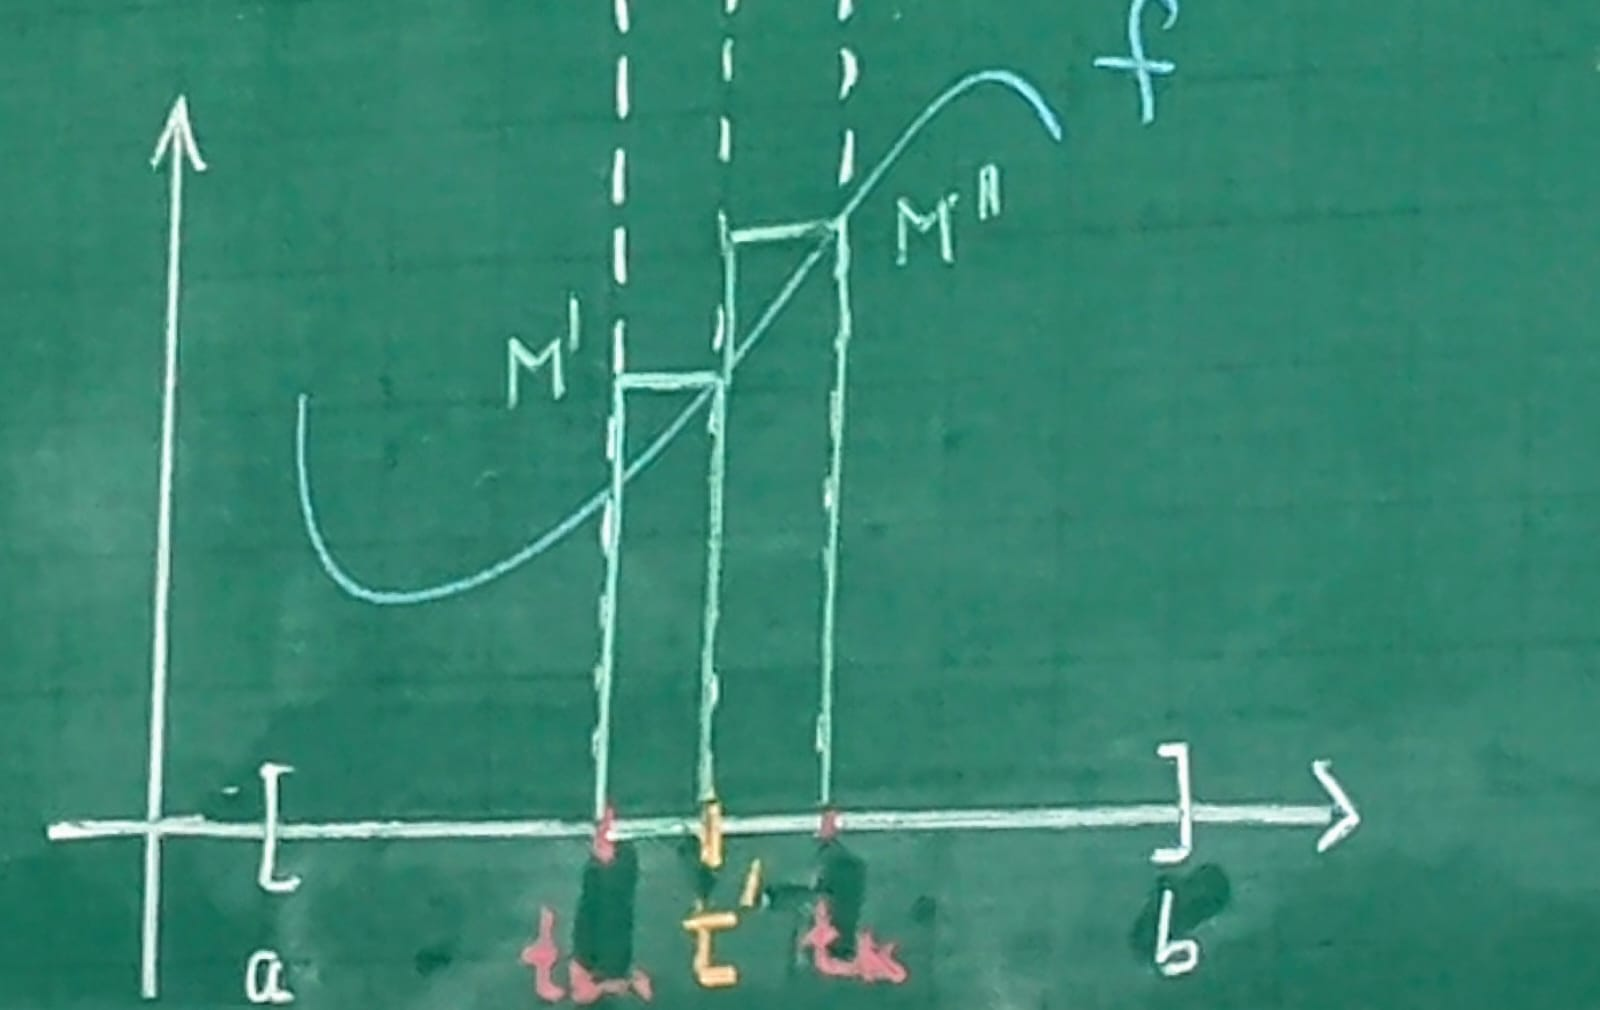
\includegraphics[height=0.4\textheight, width=0.4\textwidth, keepaspectratio]{./Images/proof_i_03.png}
		\end{center}
		\caption{Separação do subintervalo de acordo com M' e M''.}
		\label{proofimg03}
	\end{figure}

	Logo,
	\begin{align*}
		U(f; \mathcal{P}) & = \sum\limits_{i=1}^{n}M_{i}(t_{i}-t_{i-1})                                                         \\
		                  & = M_{1}(t_{1}-t_{0}) + \dotsc + M_{k}(t_{k}-t_{k-1}) + \dotsc + M_{n}(t_{n}-t_{n-1})                \\
		                  & = M_{1}(t_{1}-t_{0}) + \dotsc + M_{k}(t_{k}-t'+t'-t_{k-1}) + \dotsc + M_{n}(t_{n}-t_{n-1})          \\
		                  & = M_{1}(t_{1}-t_{0}) + \dotsc + M_{k}(t'-t_{k-1}) + M_{k}(t_{k}-t') + \dotsc + M_{n}(t_{n}-t_{n-1}) \\
		                  & \geq M_{1}(t_{1}-t_{0}) + \dotsc + M'(t'-t_{k-1}) + M''(t_{k}-t') + \dotsc + M_{n}(t_{n}-t_{n-1})   \\
		                  & = U(f; \mathcal{Q}).
	\end{align*}

	Em suma, a soma superior com respeito à partição \(\mathcal{P}\) ficou maior do que a com respeito ao refinamento \(\mathcal{Q}\).

	Na segunda etapa, consideramos um refinamento no qual foram acrescentados um número finito de pontos, isto é,
	\[
		\mathcal{Q} = \mathcal{P}\cup \{s_{1}, s_{2}, \dotsc , s_{\ell }\}
	\]
	e, do caso já provado, temos a cadeia de desigualdades
	\[
		U(f; \mathcal{P}) \geq U(f; \mathcal{P}\cup \{s_{1}\}) \geq U(f; \mathcal{P}\cup \{s_1, s_2\}) \geq \dotsc \geq U(f; \mathcal{P}\cup \{s_1, \dotsc , s_{\ell }\}) = U(f; \mathcal{Q}),
	\]
	provando, portanto, o teorema. \qedsymbol
\end{proof*}
\begin{exr}
	Refaça a prova, mas para as somas inferiores: prove o item 2.
\end{exr}

\end{document}
